\documentclass[twoside]{book}

% Packages required by doxygen
\usepackage{fixltx2e}
\usepackage{calc}
\usepackage{doxygen}
\usepackage[export]{adjustbox} % also loads graphicx
\usepackage{graphicx}
\usepackage[utf8]{inputenc}
\usepackage{makeidx}
\usepackage{multicol}
\usepackage{multirow}
\PassOptionsToPackage{warn}{textcomp}
\usepackage{textcomp}
\usepackage[nointegrals]{wasysym}
\usepackage[table]{xcolor}

% NLS support packages
\usepackage{polski}
\usepackage[T1]{fontenc}

% Font selection
\usepackage[T1]{fontenc}
\usepackage[scaled=.90]{helvet}
\usepackage{courier}
\usepackage{amssymb}
\usepackage{sectsty}
\renewcommand{\familydefault}{\sfdefault}
\allsectionsfont{%
  \fontseries{bc}\selectfont%
  \color{darkgray}%
}
\renewcommand{\DoxyLabelFont}{%
  \fontseries{bc}\selectfont%
  \color{darkgray}%
}
\newcommand{\+}{\discretionary{\mbox{\scriptsize$\hookleftarrow$}}{}{}}

% Page & text layout
\usepackage{geometry}
\geometry{%
  a4paper,%
  top=2.5cm,%
  bottom=2.5cm,%
  left=2.5cm,%
  right=2.5cm%
}
\tolerance=750
\hfuzz=15pt
\hbadness=750
\setlength{\emergencystretch}{15pt}
\setlength{\parindent}{0cm}
\setlength{\parskip}{3ex plus 2ex minus 2ex}
\makeatletter
\renewcommand{\paragraph}{%
  \@startsection{paragraph}{4}{0ex}{-1.0ex}{1.0ex}{%
    \normalfont\normalsize\bfseries\SS@parafont%
  }%
}
\renewcommand{\subparagraph}{%
  \@startsection{subparagraph}{5}{0ex}{-1.0ex}{1.0ex}{%
    \normalfont\normalsize\bfseries\SS@subparafont%
  }%
}
\makeatother

% Headers & footers
\usepackage{fancyhdr}
\pagestyle{fancyplain}
\fancyhead[LE]{\fancyplain{}{\bfseries\thepage}}
\fancyhead[CE]{\fancyplain{}{}}
\fancyhead[RE]{\fancyplain{}{\bfseries\leftmark}}
\fancyhead[LO]{\fancyplain{}{\bfseries\rightmark}}
\fancyhead[CO]{\fancyplain{}{}}
\fancyhead[RO]{\fancyplain{}{\bfseries\thepage}}
\fancyfoot[LE]{\fancyplain{}{}}
\fancyfoot[CE]{\fancyplain{}{}}
\fancyfoot[RE]{\fancyplain{}{\bfseries\scriptsize Wygenerowano przez Doxygen }}
\fancyfoot[LO]{\fancyplain{}{\bfseries\scriptsize Wygenerowano przez Doxygen }}
\fancyfoot[CO]{\fancyplain{}{}}
\fancyfoot[RO]{\fancyplain{}{}}
\renewcommand{\footrulewidth}{0.4pt}
\renewcommand{\chaptermark}[1]{%
  \markboth{#1}{}%
}
\renewcommand{\sectionmark}[1]{%
  \markright{\thesection\ #1}%
}

% Indices & bibliography
\usepackage{natbib}
\usepackage[titles]{tocloft}
\setcounter{tocdepth}{3}
\setcounter{secnumdepth}{5}
\makeindex

% Hyperlinks (required, but should be loaded last)
\usepackage{ifpdf}
\ifpdf
  \usepackage[pdftex,pagebackref=true]{hyperref}
\else
  \usepackage[ps2pdf,pagebackref=true]{hyperref}
\fi
\hypersetup{%
  colorlinks=true,%
  linkcolor=blue,%
  citecolor=blue,%
  unicode%
}

% Custom commands
\newcommand{\clearemptydoublepage}{%
  \newpage{\pagestyle{empty}\cleardoublepage}%
}

\usepackage{caption}
\captionsetup{labelsep=space,justification=centering,font={bf},singlelinecheck=off,skip=4pt,position=top}

%===== C O N T E N T S =====

\begin{document}

% Titlepage & ToC
\hypersetup{pageanchor=false,
             bookmarksnumbered=true,
             pdfencoding=unicode
            }
\pagenumbering{roman}
\begin{titlepage}
\vspace*{7cm}
\begin{center}%
{\Large Klinika zwierzat \\[1ex]\large 1 }\\
\vspace*{1cm}
{\large Wygenerowano przez Doxygen 1.8.11}\\
\end{center}
\end{titlepage}
\clearemptydoublepage
\tableofcontents
\clearemptydoublepage
\pagenumbering{arabic}
\hypersetup{pageanchor=true}

%--- Begin generated contents ---
\chapter{Indeks hierarchiczny}
\section{Hierarchia klas}
Ta lista dziedziczenia posortowana jest z grubsza, choć nie całkowicie, alfabetycznie\+:\begin{DoxyCompactList}
\item \contentsline{section}{Klinika}{\pageref{class_klinika}}{}
\item \contentsline{section}{Zwierzak}{\pageref{class_zwierzak}}{}
\begin{DoxyCompactList}
\item \contentsline{section}{G\+R\+Y\+Z\+ON}{\pageref{class_g_r_y_z_o_n}}{}
\item \contentsline{section}{K\+OT}{\pageref{class_k_o_t}}{}
\item \contentsline{section}{P\+I\+ES}{\pageref{class_p_i_e_s}}{}
\end{DoxyCompactList}
\end{DoxyCompactList}

\chapter{Indeks klas}
\section{Lista klas}
Tutaj znajdują się klasy, struktury, unie i interfejsy wraz z ich krótkimi opisami\+:\begin{DoxyCompactList}
\item\contentsline{section}{\hyperlink{class_g_r_y_z_o_n}{G\+R\+Y\+Z\+ON} }{\pageref{class_g_r_y_z_o_n}}{}
\item\contentsline{section}{\hyperlink{class_klinika}{Klinika} }{\pageref{class_klinika}}{}
\item\contentsline{section}{\hyperlink{class_k_o_t}{K\+OT} }{\pageref{class_k_o_t}}{}
\item\contentsline{section}{\hyperlink{class_p_i_e_s}{P\+I\+ES} }{\pageref{class_p_i_e_s}}{}
\item\contentsline{section}{\hyperlink{class_zwierzak}{Zwierzak} }{\pageref{class_zwierzak}}{}
\end{DoxyCompactList}

\chapter{Dokumentacja klas}
\hypertarget{class_g_r_y_z_o_n}{}\section{Dokumentacja klasy G\+R\+Y\+Z\+ON}
\label{class_g_r_y_z_o_n}\index{G\+R\+Y\+Z\+ON@{G\+R\+Y\+Z\+ON}}


{\ttfamily \#include $<$G\+R\+Y\+Z\+O\+N.\+h$>$}

Diagram dziedziczenia dla G\+R\+Y\+Z\+ON\begin{figure}[H]
\begin{center}
\leavevmode
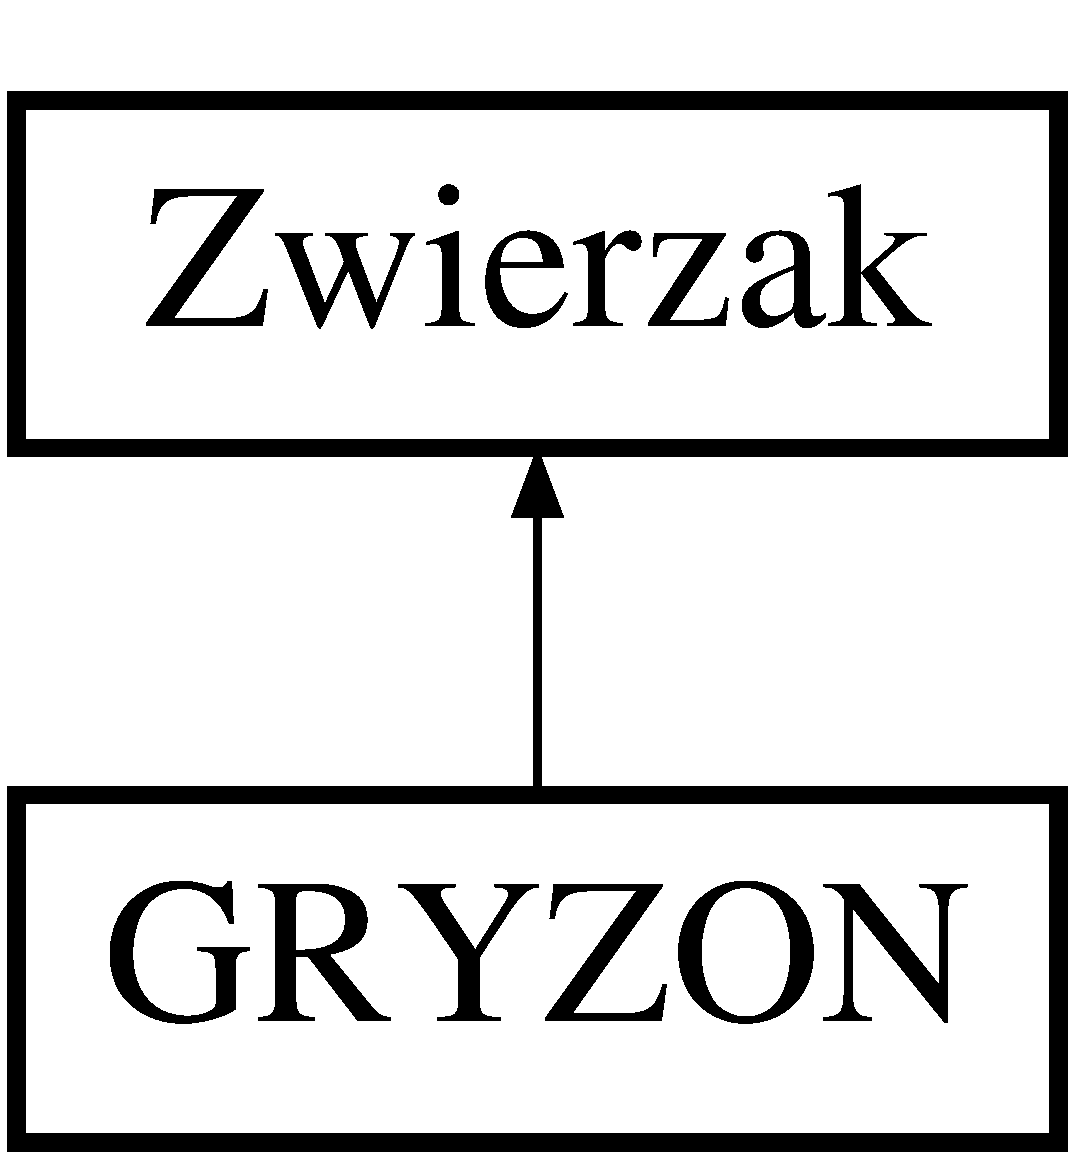
\includegraphics[height=2.000000cm]{class_g_r_y_z_o_n}
\end{center}
\end{figure}
\subsection*{Metody publiczne}
\begin{DoxyCompactItemize}
\item 
void \hyperlink{class_g_r_y_z_o_n_a4babc7ea34792cabce0ef8808f2d6a3f}{zaszczep\+\_\+gryzonia} ()
\item 
{\bfseries G\+R\+Y\+Z\+ON} (string, int, int)\hypertarget{class_g_r_y_z_o_n_a0806976434128749d7f261822432c373}{}\label{class_g_r_y_z_o_n_a0806976434128749d7f261822432c373}

\end{DoxyCompactItemize}
\subsection*{Atrybuty publiczne}
\begin{DoxyCompactItemize}
\item 
string {\bfseries rasa\+\_\+gryzonia}\hypertarget{class_g_r_y_z_o_n_a767bcc23a0f4fee52131c184743b17bf}{}\label{class_g_r_y_z_o_n_a767bcc23a0f4fee52131c184743b17bf}

\end{DoxyCompactItemize}


\subsection{Opis szczegółowy}
Project Untitled 

\subsection{Dokumentacja funkcji składowych}
\index{G\+R\+Y\+Z\+ON@{G\+R\+Y\+Z\+ON}!zaszczep\+\_\+gryzonia@{zaszczep\+\_\+gryzonia}}
\index{zaszczep\+\_\+gryzonia@{zaszczep\+\_\+gryzonia}!G\+R\+Y\+Z\+ON@{G\+R\+Y\+Z\+ON}}
\subsubsection[{\texorpdfstring{zaszczep\+\_\+gryzonia()}{zaszczep_gryzonia()}}]{\setlength{\rightskip}{0pt plus 5cm}void G\+R\+Y\+Z\+O\+N\+::zaszczep\+\_\+gryzonia (
\begin{DoxyParamCaption}
{}
\end{DoxyParamCaption}
)}\hypertarget{class_g_r_y_z_o_n_a4babc7ea34792cabce0ef8808f2d6a3f}{}\label{class_g_r_y_z_o_n_a4babc7ea34792cabce0ef8808f2d6a3f}
Project Untitled \hyperlink{class_g_r_y_z_o_n}{G\+R\+Y\+Z\+ON} implementation 

Dokumentacja dla tej klasy została wygenerowana z plików\+:\begin{DoxyCompactItemize}
\item 
G\+R\+Y\+Z\+O\+N.\+h\item 
G\+R\+Y\+Z\+O\+N.\+cpp\end{DoxyCompactItemize}

\hypertarget{class_klinika}{}\section{Dokumentacja klasy Klinika}
\label{class_klinika}\index{Klinika@{Klinika}}
\subsection*{Metody publiczne}
\begin{DoxyCompactItemize}
\item 
void \hyperlink{class_klinika_a2a0a9fc98c983c444ecd3d3056d6b7cc}{dodaj} (\hyperlink{class_zwierzak}{Zwierzak} \&)
\item 
void {\bfseries usun} ()\hypertarget{class_klinika_a9061d14ca355d8b862bdfb80b90cbf09}{}\label{class_klinika_a9061d14ca355d8b862bdfb80b90cbf09}

\item 
void {\bfseries wyszukaj} ()\hypertarget{class_klinika_a8ba3d0d069914516b476cdfde0479905}{}\label{class_klinika_a8ba3d0d069914516b476cdfde0479905}

\item 
void {\bfseries wyswietl} ()\hypertarget{class_klinika_a2d8f47cd4d1d2a74e006c9117fe40786}{}\label{class_klinika_a2d8f47cd4d1d2a74e006c9117fe40786}

\end{DoxyCompactItemize}
\subsection*{Atrybuty publiczne}
\begin{DoxyCompactItemize}
\item 
list$<$ \hyperlink{class_zwierzak}{Zwierzak} $>$ {\bfseries lista\+\_\+zwierzat}\hypertarget{class_klinika_a16fb2af6cf2590908b68ebf4ec99bb37}{}\label{class_klinika_a16fb2af6cf2590908b68ebf4ec99bb37}

\item 
string {\bfseries Nazwa} = \char`\"{}Bari\char`\"{}\hypertarget{class_klinika_af7c4fbb622fb15c5fd4e1bca1631d3d1}{}\label{class_klinika_af7c4fbb622fb15c5fd4e1bca1631d3d1}

\item 
string {\bfseries Ulica} = \char`\"{} Komsmowskiego 2\char`\"{}\hypertarget{class_klinika_a58f8f674729da531a7a7598d10425674}{}\label{class_klinika_a58f8f674729da531a7a7598d10425674}

\item 
int {\bfseries numer} = 24\hypertarget{class_klinika_a1041634c81e611fb7a892b36c525e32d}{}\label{class_klinika_a1041634c81e611fb7a892b36c525e32d}

\end{DoxyCompactItemize}


\subsection{Dokumentacja funkcji składowych}
\index{Klinika@{Klinika}!dodaj@{dodaj}}
\index{dodaj@{dodaj}!Klinika@{Klinika}}
\subsubsection[{\texorpdfstring{dodaj(\+Zwierzak \&)}{dodaj(Zwierzak &)}}]{\setlength{\rightskip}{0pt plus 5cm}void Klinika\+::dodaj (
\begin{DoxyParamCaption}
\item[{{\bf Zwierzak} \&}]{pacjent}
\end{DoxyParamCaption}
)}\hypertarget{class_klinika_a2a0a9fc98c983c444ecd3d3056d6b7cc}{}\label{class_klinika_a2a0a9fc98c983c444ecd3d3056d6b7cc}
Project Untitled \hyperlink{class_klinika}{Klinika} implementation 

Dokumentacja dla tej klasy została wygenerowana z plików\+:\begin{DoxyCompactItemize}
\item 
Klinika.\+h\item 
Klinika.\+cpp\end{DoxyCompactItemize}

\hypertarget{class_k_o_t}{}\section{Dokumentacja klasy K\+OT}
\label{class_k_o_t}\index{K\+OT@{K\+OT}}


{\ttfamily \#include $<$K\+O\+T.\+h$>$}

Diagram dziedziczenia dla K\+OT\begin{figure}[H]
\begin{center}
\leavevmode
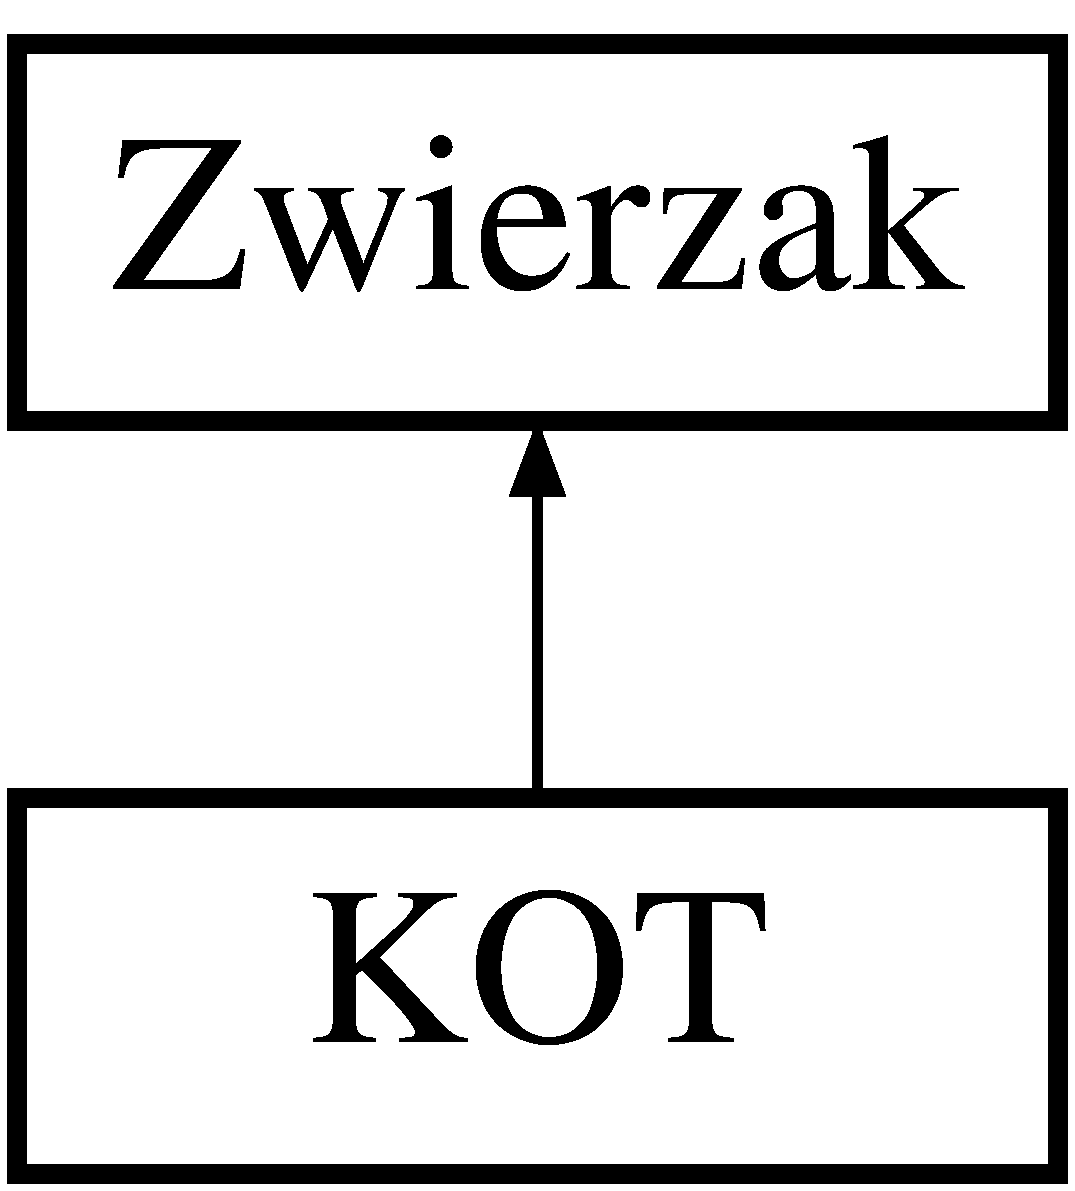
\includegraphics[height=2.000000cm]{class_k_o_t}
\end{center}
\end{figure}
\subsection*{Metody publiczne}
\begin{DoxyCompactItemize}
\item 
void \hyperlink{class_k_o_t_a7ef8cd0d3488f4c96e071b2722e77cab}{zaszczep\+\_\+kota} ()
\item 
{\bfseries K\+OT} (string imie, int wiek, int waga)\hypertarget{class_k_o_t_aecdfea3a5fb53138d45c6afa63ce7704}{}\label{class_k_o_t_aecdfea3a5fb53138d45c6afa63ce7704}

\end{DoxyCompactItemize}
\subsection*{Atrybuty publiczne}
\begin{DoxyCompactItemize}
\item 
string {\bfseries rasa\+\_\+kota}\hypertarget{class_k_o_t_a7e2211bfeca89ce0d6640db13d2a4182}{}\label{class_k_o_t_a7e2211bfeca89ce0d6640db13d2a4182}

\end{DoxyCompactItemize}


\subsection{Opis szczegółowy}
Project Untitled 

\subsection{Dokumentacja funkcji składowych}
\index{K\+OT@{K\+OT}!zaszczep\+\_\+kota@{zaszczep\+\_\+kota}}
\index{zaszczep\+\_\+kota@{zaszczep\+\_\+kota}!K\+OT@{K\+OT}}
\subsubsection[{\texorpdfstring{zaszczep\+\_\+kota()}{zaszczep_kota()}}]{\setlength{\rightskip}{0pt plus 5cm}void K\+O\+T\+::zaszczep\+\_\+kota (
\begin{DoxyParamCaption}
{}
\end{DoxyParamCaption}
)}\hypertarget{class_k_o_t_a7ef8cd0d3488f4c96e071b2722e77cab}{}\label{class_k_o_t_a7ef8cd0d3488f4c96e071b2722e77cab}
\hyperlink{class_k_o_t}{K\+OT} implementation 

Dokumentacja dla tej klasy została wygenerowana z plików\+:\begin{DoxyCompactItemize}
\item 
K\+O\+T.\+h\item 
K\+O\+T.\+cpp\end{DoxyCompactItemize}

\hypertarget{class_p_i_e_s}{}\section{Dokumentacja klasy P\+I\+ES}
\label{class_p_i_e_s}\index{P\+I\+ES@{P\+I\+ES}}


{\ttfamily \#include $<$P\+I\+E\+S.\+h$>$}

Diagram dziedziczenia dla P\+I\+ES\begin{figure}[H]
\begin{center}
\leavevmode
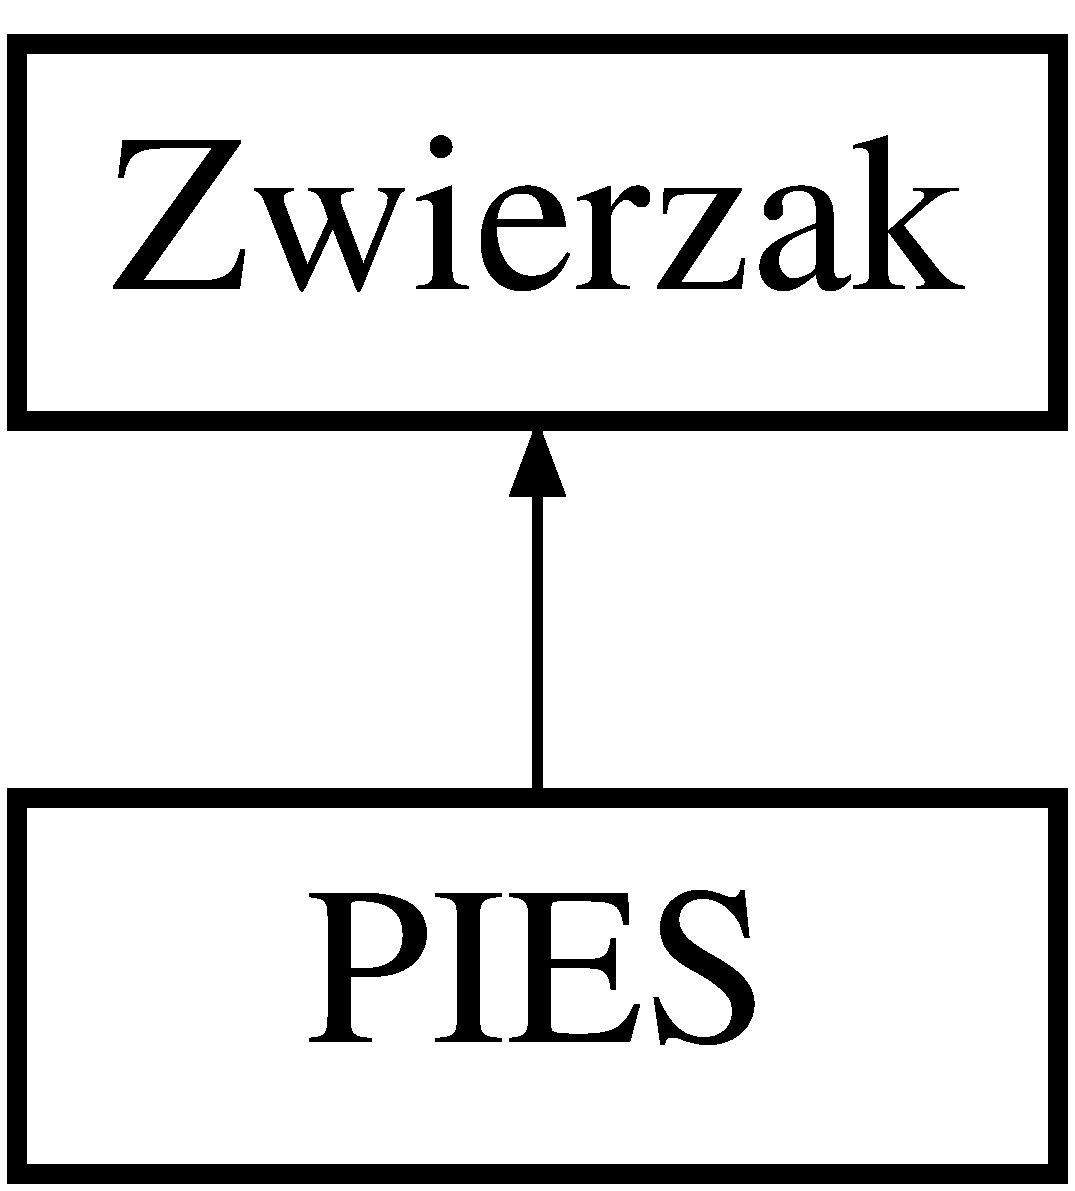
\includegraphics[height=2.000000cm]{class_p_i_e_s}
\end{center}
\end{figure}
\subsection*{Metody publiczne}
\begin{DoxyCompactItemize}
\item 
\hyperlink{class_p_i_e_s_aa11f80bdbaee36f20c312b6f17fc7f9c}{P\+I\+ES} ()
\item 
{\bfseries P\+I\+ES} (string, int, int)\hypertarget{class_p_i_e_s_aa24a5012c7396d03ad506a430bfec167}{}\label{class_p_i_e_s_aa24a5012c7396d03ad506a430bfec167}

\item 
void {\bfseries zaszczep\+\_\+psa} ()\hypertarget{class_p_i_e_s_a59254ad3c8094174cb7d1b0fe330b4b2}{}\label{class_p_i_e_s_a59254ad3c8094174cb7d1b0fe330b4b2}

\end{DoxyCompactItemize}
\subsection*{Atrybuty publiczne}
\begin{DoxyCompactItemize}
\item 
string {\bfseries rasa\+\_\+psa}\hypertarget{class_p_i_e_s_a12202e02d4945d1ffda8770e86571df6}{}\label{class_p_i_e_s_a12202e02d4945d1ffda8770e86571df6}

\end{DoxyCompactItemize}


\subsection{Opis szczegółowy}
Project Untitled 

\subsection{Dokumentacja konstruktora i destruktora}
\index{P\+I\+ES@{P\+I\+ES}!P\+I\+ES@{P\+I\+ES}}
\index{P\+I\+ES@{P\+I\+ES}!P\+I\+ES@{P\+I\+ES}}
\subsubsection[{\texorpdfstring{P\+I\+E\+S()}{PIES()}}]{\setlength{\rightskip}{0pt plus 5cm}P\+I\+E\+S\+::\+P\+I\+ES (
\begin{DoxyParamCaption}
{}
\end{DoxyParamCaption}
)}\hypertarget{class_p_i_e_s_aa11f80bdbaee36f20c312b6f17fc7f9c}{}\label{class_p_i_e_s_aa11f80bdbaee36f20c312b6f17fc7f9c}
Project Untitled \hyperlink{class_p_i_e_s}{P\+I\+ES} implementation 

Dokumentacja dla tej klasy została wygenerowana z plików\+:\begin{DoxyCompactItemize}
\item 
P\+I\+E\+S.\+h\item 
P\+I\+E\+S.\+cpp\end{DoxyCompactItemize}

\hypertarget{class_zwierzak}{}\section{Dokumentacja klasy Zwierzak}
\label{class_zwierzak}\index{Zwierzak@{Zwierzak}}
Diagram dziedziczenia dla Zwierzak\begin{figure}[H]
\begin{center}
\leavevmode
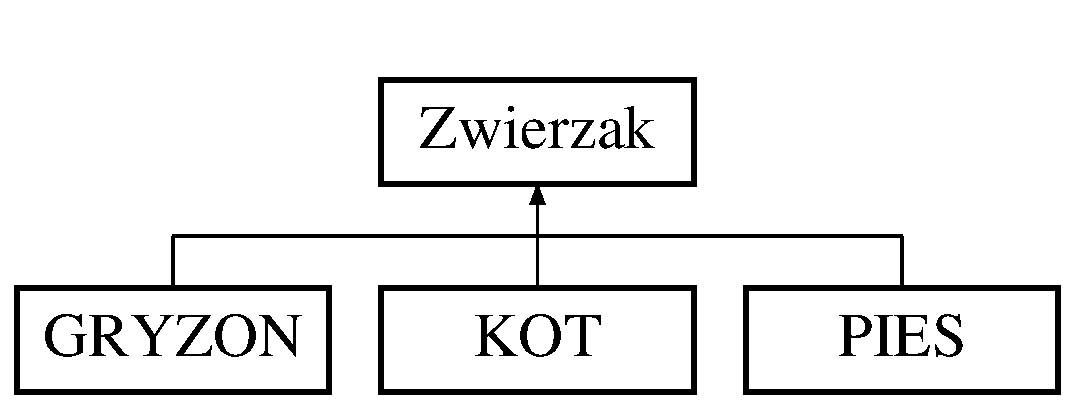
\includegraphics[height=2.000000cm]{class_zwierzak}
\end{center}
\end{figure}
\subsection*{Metody publiczne}
\begin{DoxyCompactItemize}
\item 
{\bfseries Zwierzak} (string im\+\_\+pacjenta, int nr\+\_\+pac, int w, int wag, bool sz)\hypertarget{class_zwierzak_a60705f18b6910541acfeb6ba2fb8d049}{}\label{class_zwierzak_a60705f18b6910541acfeb6ba2fb8d049}

\end{DoxyCompactItemize}
\subsection*{Atrybuty publiczne}
\begin{DoxyCompactItemize}
\item 
string {\bfseries imie}\hypertarget{class_zwierzak_a0a32e3dccc1bbfce4e192bad8957e0eb}{}\label{class_zwierzak_a0a32e3dccc1bbfce4e192bad8957e0eb}

\item 
int {\bfseries nr\+\_\+\+ID}\hypertarget{class_zwierzak_a49ae8dd3b765af187014cdd79d554880}{}\label{class_zwierzak_a49ae8dd3b765af187014cdd79d554880}

\item 
int {\bfseries wiek}\hypertarget{class_zwierzak_ace4be3289ee2cea5aaf441233c5df999}{}\label{class_zwierzak_ace4be3289ee2cea5aaf441233c5df999}

\item 
int {\bfseries waga}\hypertarget{class_zwierzak_acd4b5b7d45ab6dbcb20810bf6d0b91ca}{}\label{class_zwierzak_acd4b5b7d45ab6dbcb20810bf6d0b91ca}

\item 
bool {\bfseries szczepienie}\hypertarget{class_zwierzak_ac77058255f281fa40fa21e81257f1104}{}\label{class_zwierzak_ac77058255f281fa40fa21e81257f1104}

\end{DoxyCompactItemize}


Dokumentacja dla tej klasy została wygenerowana z pliku\+:\begin{DoxyCompactItemize}
\item 
Zwierzak.\+h\end{DoxyCompactItemize}

%--- End generated contents ---

% Index
\backmatter
\newpage
\phantomsection
\clearemptydoublepage
\addcontentsline{toc}{chapter}{Indeks}
\printindex

\end{document}
